\documentclass[letterpaper, 10 pt, conference]{ieeeconf}
\overrideIEEEmargins
\IEEEoverridecommandlockouts
\usepackage{times}
\usepackage{multicol}
\usepackage{graphicx}
\usepackage{xcolor}
\usepackage{booktabs}
\usepackage{amsmath}
\usepackage{amssymb}
\usepackage{url}
\usepackage{hyperref}
\hypersetup{colorlinks=true, linkcolor=black, citecolor=blue, urlcolor=blue}
\newtheorem{theorem}{Theorem}
\usepackage[algoruled,vlined,linesnumbered]{algorithm2e}
\usepackage{anyfontsize}

\title{Music Wrapped: An Interactive Music Discovery System with K-Means Personality Archetypes and Cosine-Similarity Recommendations}

\author{Jesse Boakye, Kenneth Son, Luis Zarate, Ralph Lewis \\
\textit{CPTS 315 --- Data Mining, Spring 2026, Washington State University}}

\begin{document}

\maketitle

\begin{abstract}
We present \emph{Music Wrapped}, an interactive Spotify-Wrapped-style music discovery system built around two classical data-mining techniques: K-means clustering for music-personality assignment and cosine similarity for content-based recommendation. The system uses a Kaggle Spotify catalog of 4{,}494 tracks and eight normalized audio features (danceability, energy, valence, acousticness, instrumentalness, speechiness, tempo, loudness). Users select 3--10 seed songs and receive a six-slide report covering aggregate statistics, mood, music personality, audio DNA, top recommendations, and hidden gems. K-means with $K{=}6$ on the original feature space wins over a 6-component PCA representation by a thin silhouette margin (0.252 vs.\ 0.270 within the demo-relevant K range, but reverting to original features on the interpretability tiebreaker). Six interpretable archetypes emerge from centroid analysis. Leave-one-out seed recovery on 200 simulated users yields Hit@10 of 1.6\% for genre-coherent seeds (8$\times$ random baseline, 2.4$\times$ better than random on median rank). A controlled comparison shows cosine similarity beats Euclidean distance at the high-precision end (Hit@5 +20\%, MRR +11\%) while Euclidean wins marginally in the tail. The full pipeline is implemented in Python and packaged as a Streamlit demo.
\end{abstract}

\section{Introduction}

Spotify Wrapped, the year-end personalized listening report, has become a cultural touchstone --- not because the underlying recommender is novel, but because the \emph{presentation} of audio analytics is engaging. Most class-project music recommendation systems stop at ``return the ten most-similar songs.'' We argue that pairing a content-based recommender with a Wrapped-style report --- mood, archetype, audio DNA, recommendations, and hidden gems --- produces a far stronger demo and forces a full data-mining pipeline (preprocessing, EDA, clustering, similarity, evaluation).

This work uses the Spotify Music Dataset~\cite{spotify_dataset}: a Kaggle catalog of tracks with Spotify-derived audio features, popularity, and playlist-of-origin metadata. We restrict modeling to a shared 8-feature audio set, normalized via Min--Max scaling. Two algorithms drive every downstream slide: K-means~\cite{macqueen1967kmeans} for assigning a personality archetype to a user's seed selection, and cosine similarity~\cite{singhal2001modern} for ranking recommendations against the user's average feature vector.

\emph{Statement of the question.} Given 3--10 user-selected seed songs from a static catalog, can a content-based system using K-means cluster archetypes and cosine-similarity ranking produce a recommendation experience that is (a) algorithmically defensible (better than random on standard offline metrics), (b) interpretable to a non-technical audience, and (c) worth shipping as an interactive demo?

\section{Related Work}

K-means clustering~\cite{macqueen1967kmeans} and the silhouette score~\cite{rousseeuw1987silhouettes} are the standard textbook approach to discovering interpretable groups in continuous feature data. Aggarwal's recommender-systems textbook~\cite{aggarwal2016recommender} characterizes our recommendation engine as content-based filtering with a similarity metric: cheap to compute, no cold-start problem (we always have seed songs), but limited by the expressivity of the feature set. PCA~\cite{jolliffe2016pca} is used in our pipeline strictly for visualization and as an experimental clustering input, not for the user-facing recommender, which preserves explainability via the original audio features. The scikit-learn library~\cite{pedregosa2011scikit} provides the implementations of K-means, cosine similarity, Min--Max scaling, PCA, and silhouette scoring used throughout.

\section{Problem Formulation}

\subsection{Input}

A static catalog $\mathcal{C}$ of $|\mathcal{C}|{=}4{,}494$ tracks (after concatenating two Kaggle CSV files, deduplicating by \texttt{track\_id}, and dropping rows with any missing modeling feature). Each track has eight numerical audio features in $\mathbb{R}^8$, an integer popularity score in $[0,100]$, and metadata (artist, album, playlist source, etc.). A user supplies a seed set $S \subseteq \mathcal{C}$ with $3 \leq |S| \leq 10$.

\subsection{Output}

For each seed set the system produces:
\begin{enumerate}
\item A mood label from a rule-based valence/energy classifier with thresholds tuned by EDA (high $\geq 0.6$, low-valence $< 0.35$).
\item A personality archetype label, by computing the seed's average feature vector $\bar{x} = \frac{1}{|S|}\sum_{x\in S} x$, then assigning $\bar{x}$ to its nearest K-means centroid.
\item A ranked top-10 recommendation list using a blended score $\text{final}(t) = \alpha \cdot \cos(t, \bar{x}) + (1-\alpha)\cdot \text{pop}(t)/100$, with $\alpha = 0.95$ chosen empirically (see Section~\ref{sec:alpha}).
\item A top-8 hidden-gems list: the top-decile most-similar tracks (excluding the main rec list), filtered to popularity below $\min(\text{median}(\mathcal{C}), \overline{\text{pop}}(S))$.
\item Aggregate visualizations: top genres/artists, valence/energy mood scatter, audio-DNA radar, and the cluster centroid radar.
\end{enumerate}

\subsection{Constraints}

No live API calls, no user behavior data (no listening histories, no ratings); the system is therefore content-based by necessity. Every slide must be explainable from the feature set --- this rules out using PCA components in the user-facing recommender.

\section{Algorithm and Methodology}

\begin{figure}[h]
\centering
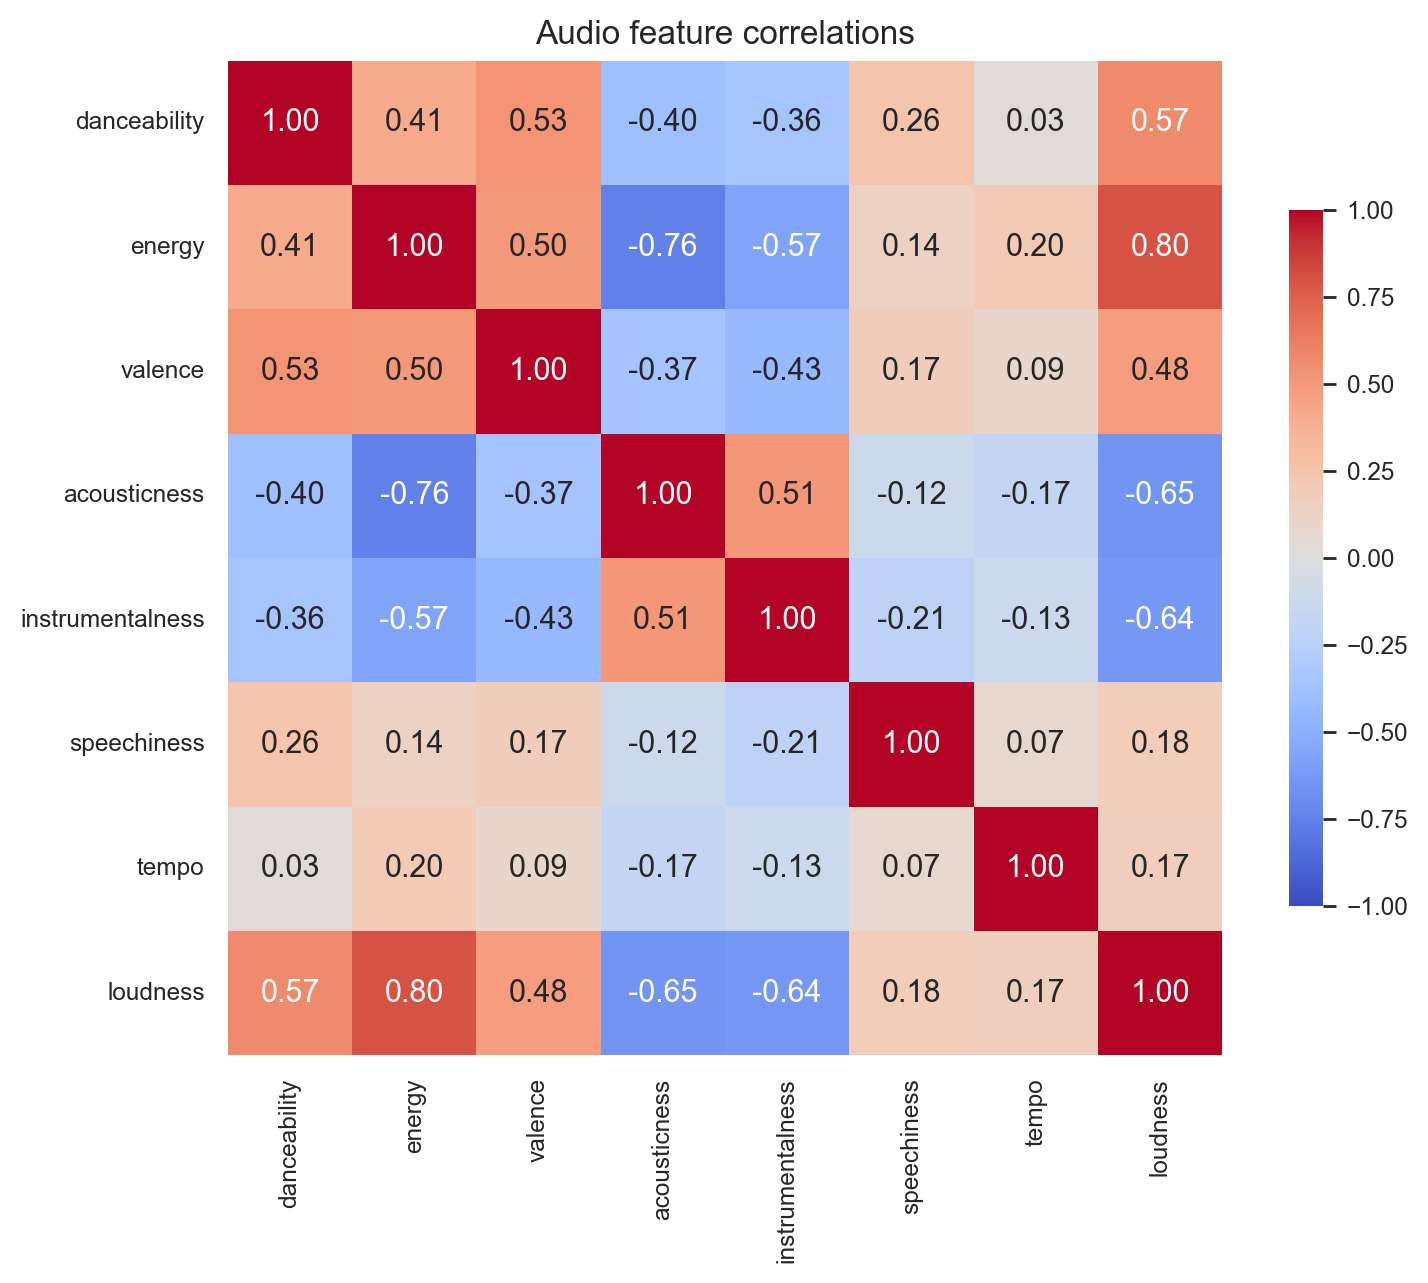
\includegraphics[width=0.46\textwidth]{figures/correlation_heatmap.png}
\caption{Audio feature correlations on the cleaned 4{,}494-track catalog. Energy/loudness correlate at $\rho{=}0.80$ and energy/acousticness at $-0.76$, motivating a PCA experiment for clustering.}
\label{fig:corr}
\end{figure}

\subsection{Preprocessing}

The two Kaggle CSVs (\texttt{high\_popularity\_spotify\_data.csv}, \texttt{low\_popularity\_spotify\_data.csv}) are concatenated, deduplicated by \texttt{track\_id}, and rows with missing modeling features are dropped. The shared eight-feature set --- danceability, energy, valence, acousticness, instrumentalness, speechiness, tempo, loudness --- is normalized to $[0,1]$ via \texttt{MinMaxScaler}. A consistent feature set across clustering and recommendation keeps results interpretable.

\subsection{Exploratory Data Analysis}

EDA (Figs.~\ref{fig:corr}, \ref{fig:dist}, \ref{fig:genre_profile}) revealed three findings that shape the rest of the pipeline:
\begin{itemize}
\item \emph{Strong feature correlations.} Energy/loudness $\rho{=}0.80$, acousticness/energy $\rho{=}-0.76$. Six PCA components capture $\geq 95\%$ of variance, motivating the PCA-vs-original clustering experiment.
\item \emph{Genre-skewed catalog.} Top genres (electronic, pop, latin, hip-hop, ambient, rock, lofi) hold 300--560 tracks each; sparse genres (disco, country, soca, mandopop) have $<30$. Sparse genres are bucketed into ``other'' for the genre-consistency metric to avoid tiny-sample noise.
\item \emph{Mood threshold tuning.} The valence$\times$energy scatter (Fig.~\ref{fig:mood}) showed all four quadrants populated, but the low-energy/high-valence corner was sparse at the textbook 0.5 split. Thresholds were retuned to high $\geq 0.6$ and low-valence $< 0.35$.
\end{itemize}

\begin{figure}[h]
\centering
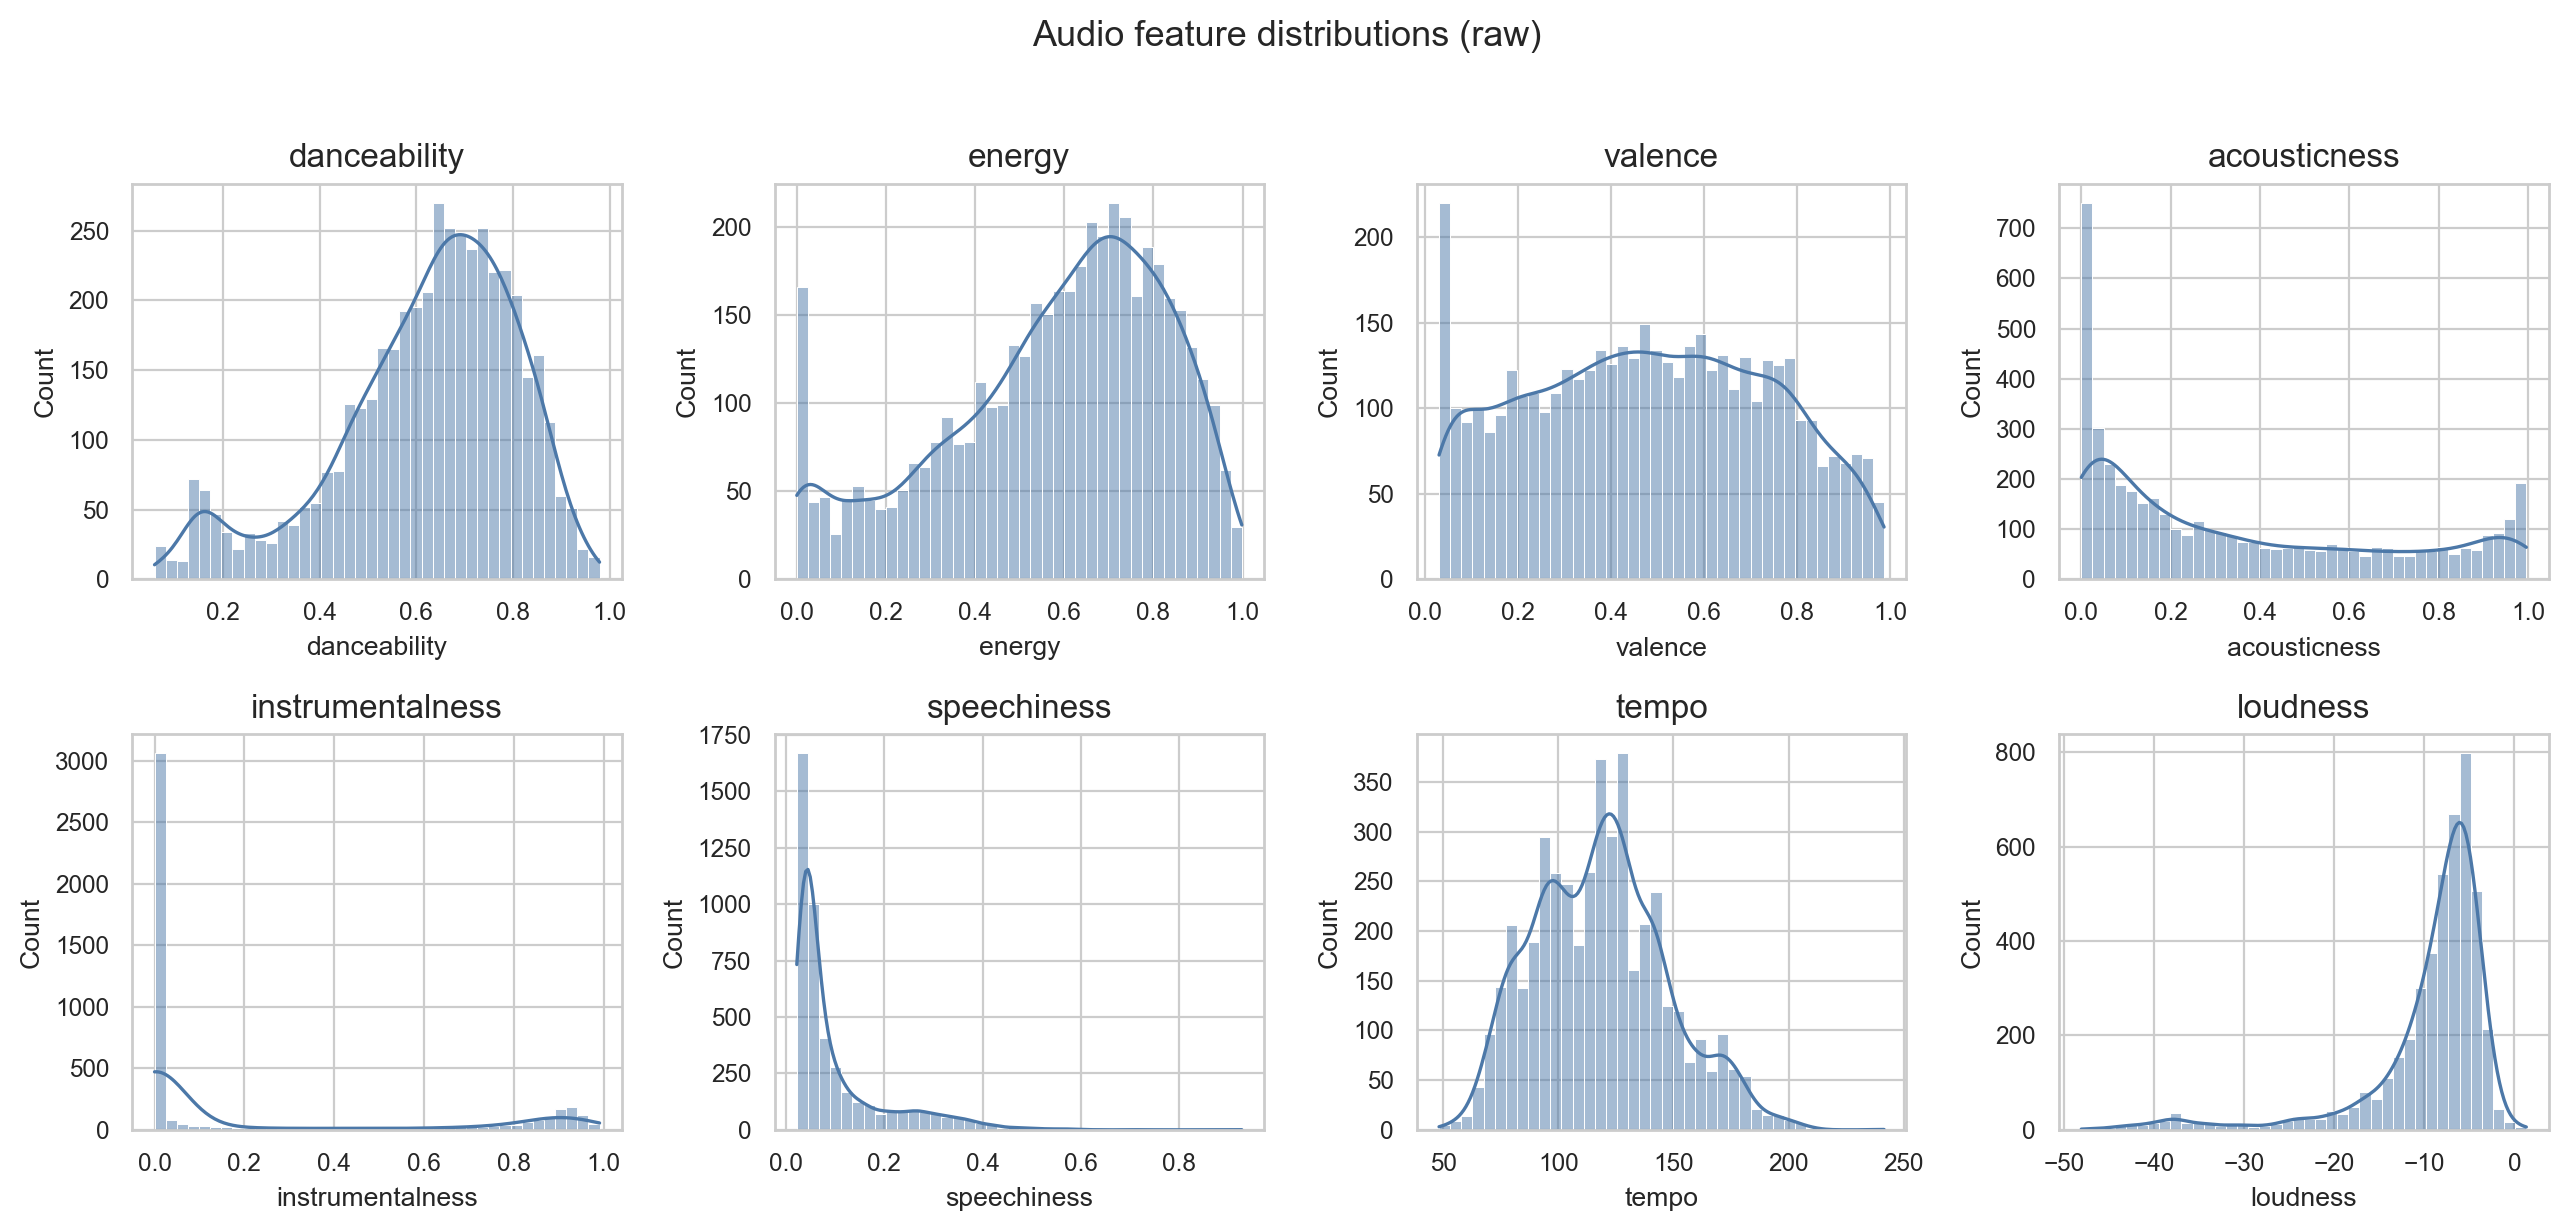
\includegraphics[width=0.48\textwidth]{figures/feature_distributions.png}
\caption{Audio feature distributions. \texttt{instrumentalness} and \texttt{speechiness} are heavy right-tailed; \texttt{tempo} centers near 118 BPM; \texttt{danceability}/\texttt{energy}/\texttt{valence} are well-spread.}
\label{fig:dist}
\end{figure}

\begin{figure}[h]
\centering
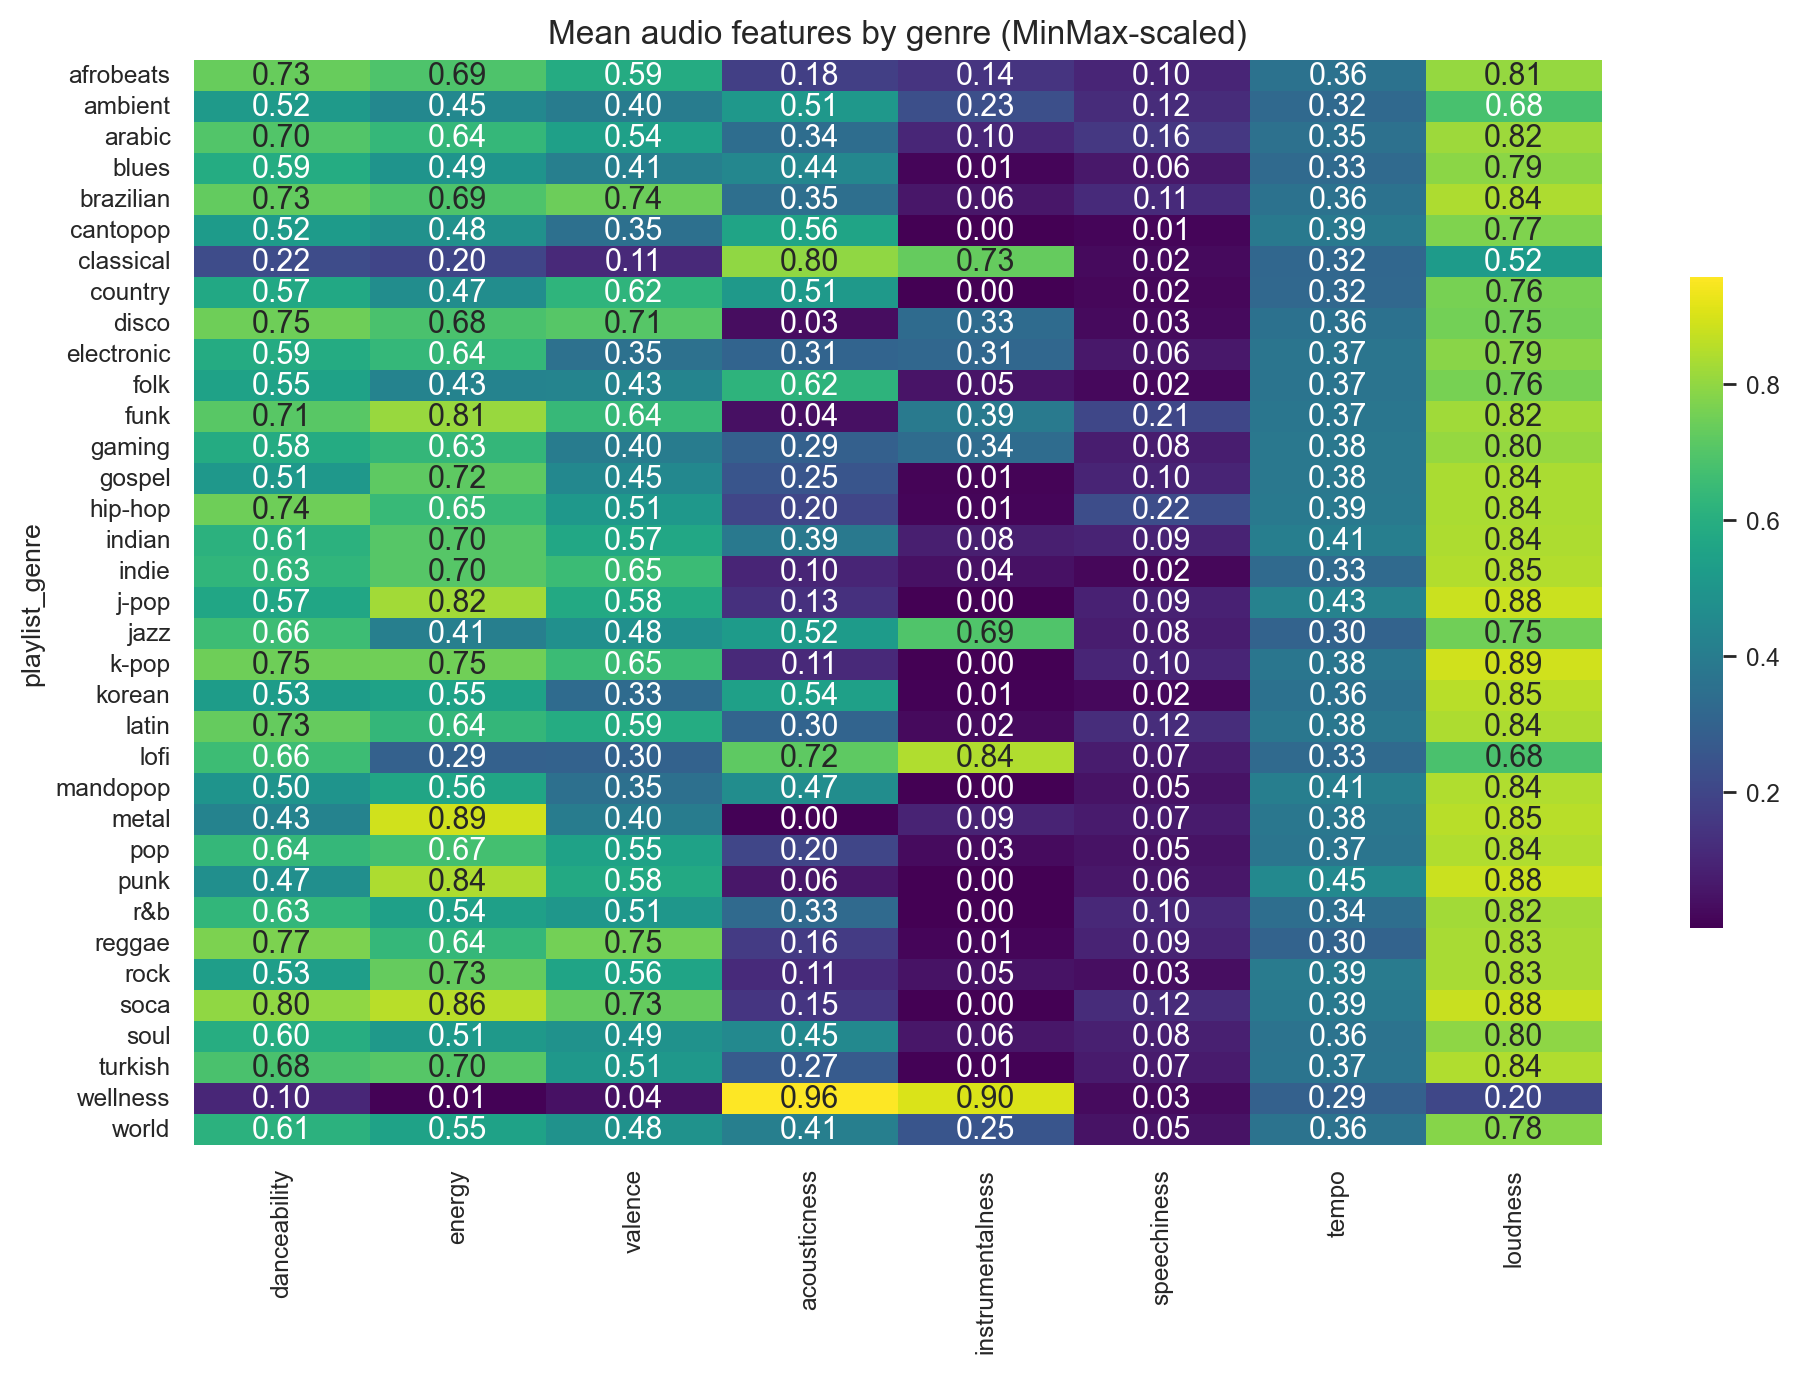
\includegraphics[width=0.48\textwidth]{figures/genre_profile_heatmap.png}
\caption{Mean MinMax-scaled audio features per genre. Wellness/classical/lofi cluster as low-energy and acoustic; metal/punk/rock as high-energy. This table seeds the cluster-archetype labeling step.}
\label{fig:genre_profile}
\end{figure}

\begin{figure}[h]
\centering
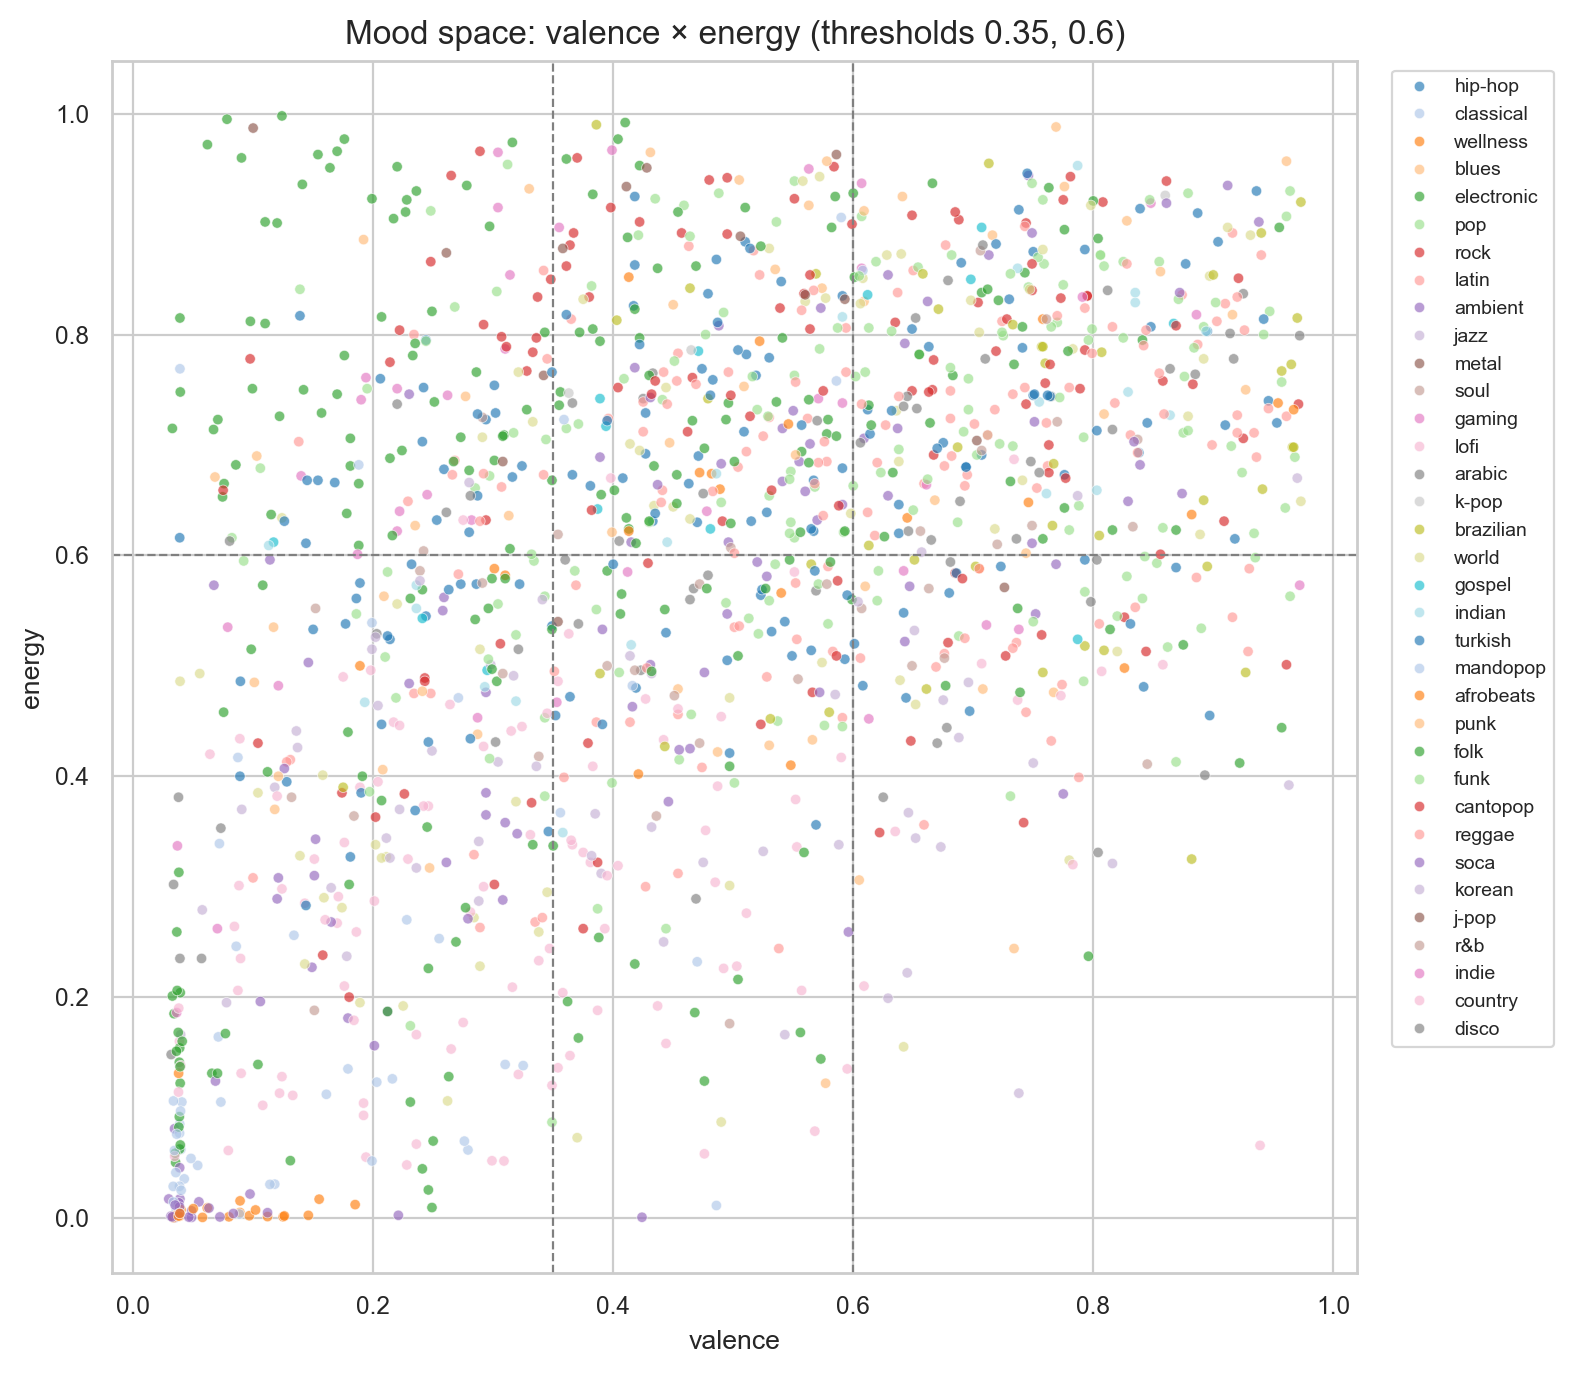
\includegraphics[width=0.48\textwidth]{figures/mood_quadrants.png}
\caption{Mood space (valence~$\times$~energy) sampled at 1{,}500 tracks. Dashed lines show the EDA-tuned mood thresholds (0.35 low-valence, 0.6 high-valence/energy).}
\label{fig:mood}
\end{figure}

\subsection{PCA Experiment}

PCA was fit on the standardized 8-feature matrix. Two dimensions explain 71\% of variance --- enough for visualization (Fig.~\ref{fig:pca}, left) but with significant genre overlap. The full cumulative-variance curve (Fig.~\ref{fig:pca}, right) shows six components hit $\geq 95\%$ variance. PCA was not used for the recommender (interpretability), but a 6-component PCA representation was tested as a clustering input.

\begin{figure}[h]
\centering
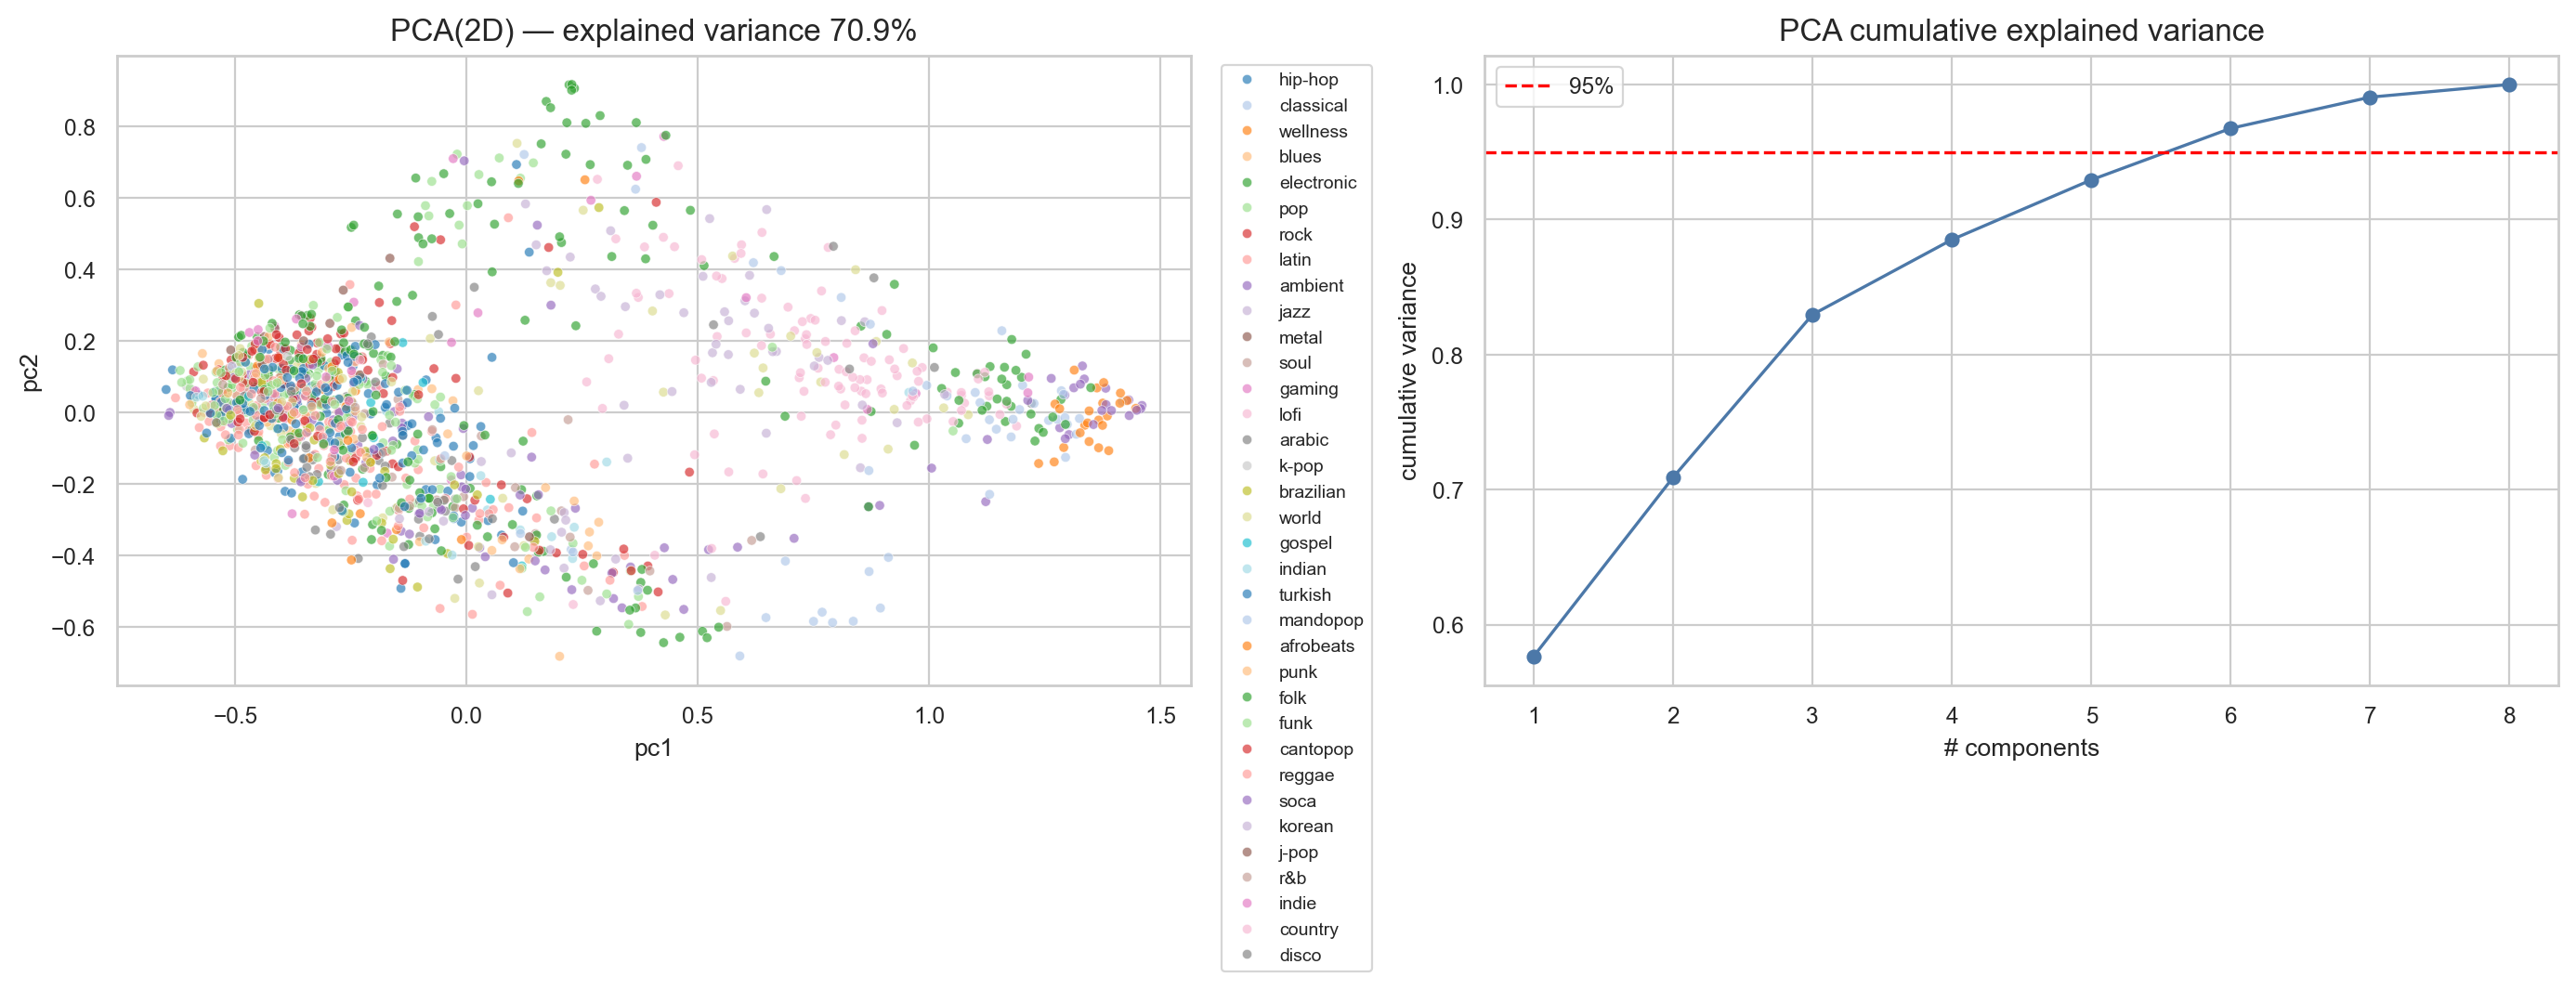
\includegraphics[width=0.48\textwidth]{figures/pca_2d_and_variance.png}
\caption{Left: PCA(2D) scatter colored by genre. Right: cumulative explained-variance curve --- 6 components reach 95\%.}
\label{fig:pca}
\end{figure}

\subsection{K-Means Clustering: Two-Track Experiment}
\label{sec:clustering}

\begin{figure}[h]
\centering
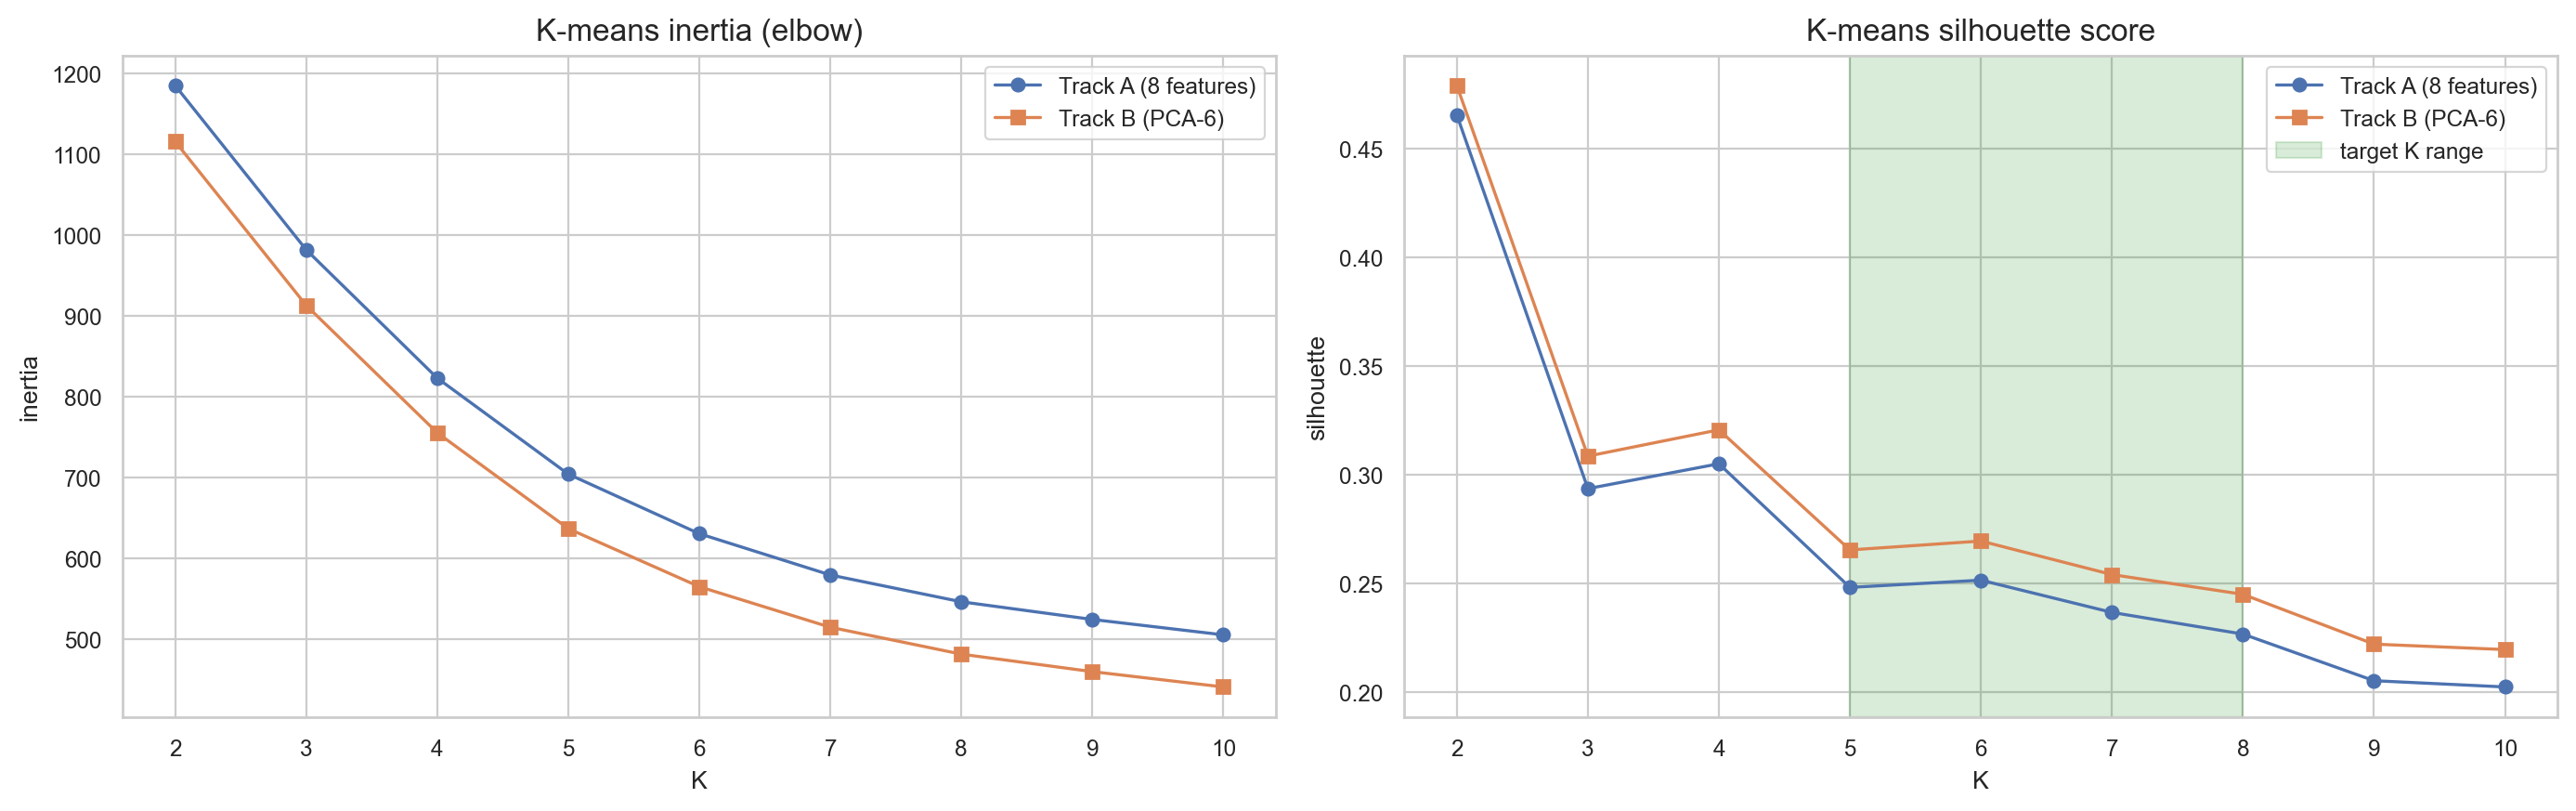
\includegraphics[width=0.48\textwidth]{figures/kmeans_elbow_silhouette.png}
\caption{K-means scans on the original 8 features (Track A) and the 6-component PCA representation (Track B). The shaded region marks the demo-relevant target range $K \in [5,8]$. Silhouette peaks at $K{=}2$ in both tracks --- a known artifact of pure silhouette maximization on overlapping data --- so the decision rule restricts to the target range.}
\label{fig:elbow}
\end{figure}

K-means was run for $K \in [2,10]$ on both representations. To avoid the well-known degenerate $K{=}2$ silhouette peak, the decision rule restricted to the demo-relevant range $K \in [5,8]$ and required that no cluster fall below 2\% of the catalog. Within that range, silhouette was 0.270 for Track B (PCA-6, $K{=}6$) and 0.252 for Track A (original features, $K{=}6$). The 0.018 difference fell inside our 0.02 interpretability-tiebreaker, so Track A won. K-means initialization was stable across five seeds (silhouette 0.2515 $\pm$ 0.0001).

\begin{figure}[h]
\centering
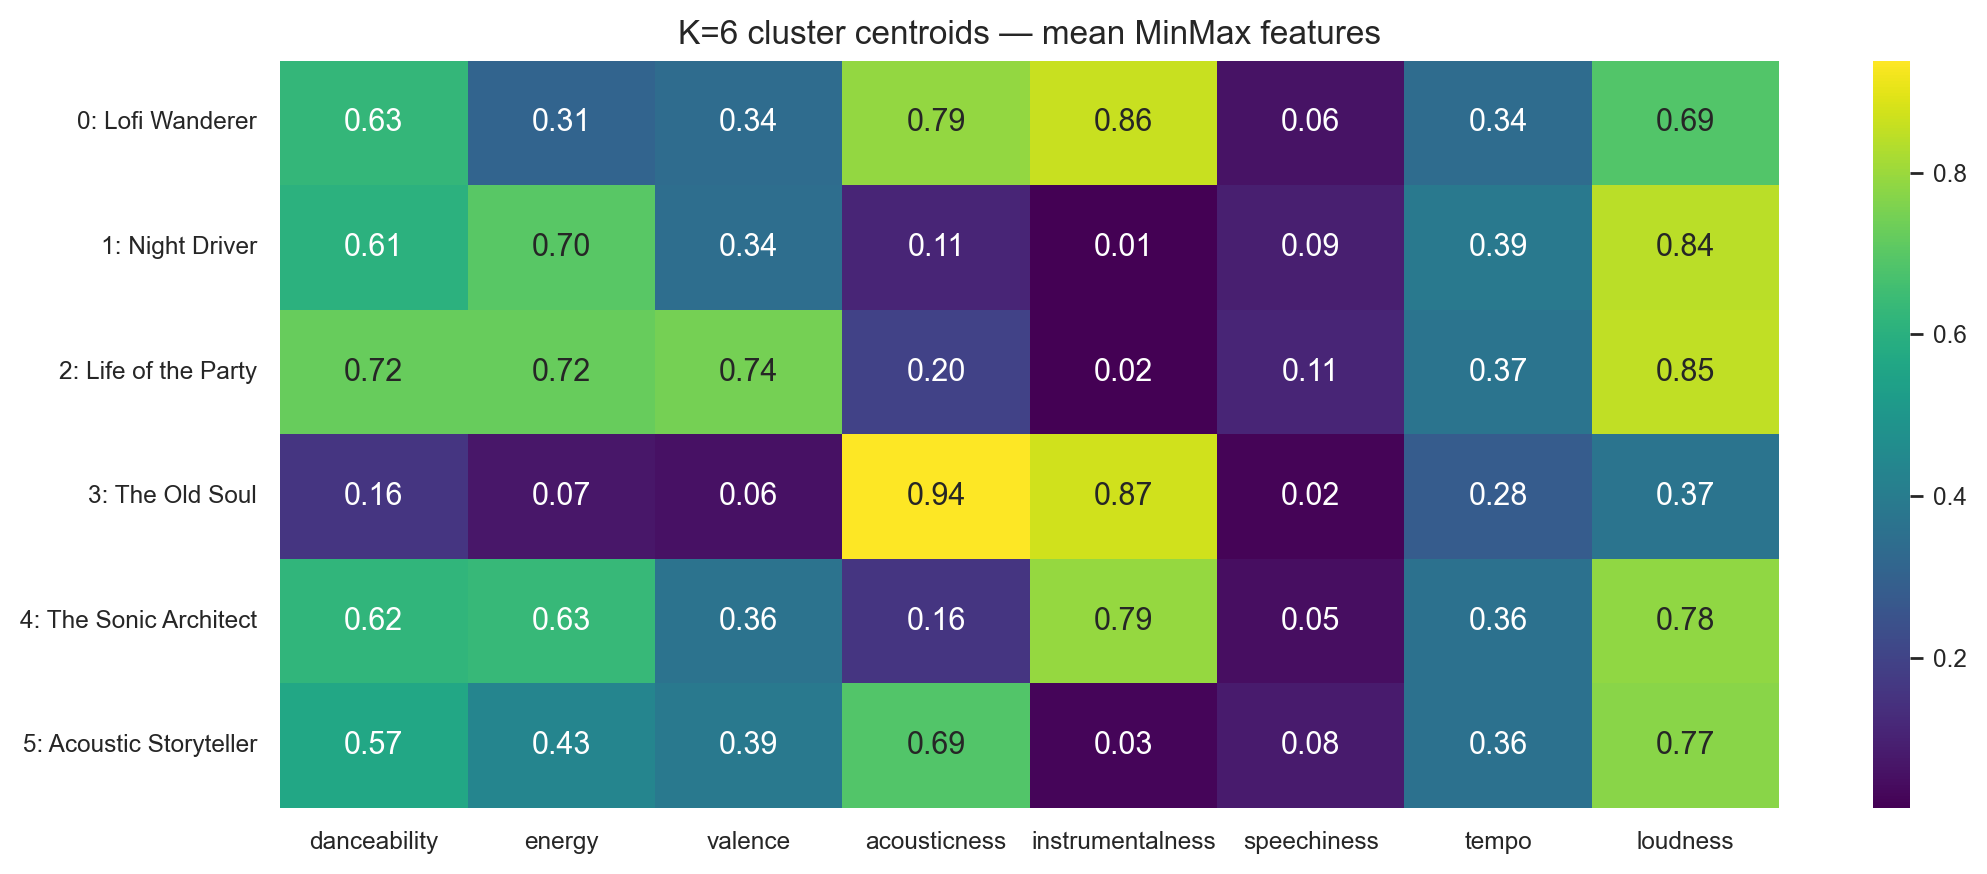
\includegraphics[width=0.48\textwidth]{figures/cluster_profile.png}
\caption{$K{=}6$ cluster centroids in the original feature space. Each row is one archetype; columns are the eight normalized audio features. Centroid analysis drives the human-readable archetype labels.}
\label{fig:cluster_profile}
\end{figure}

\begin{figure}[h]
\centering
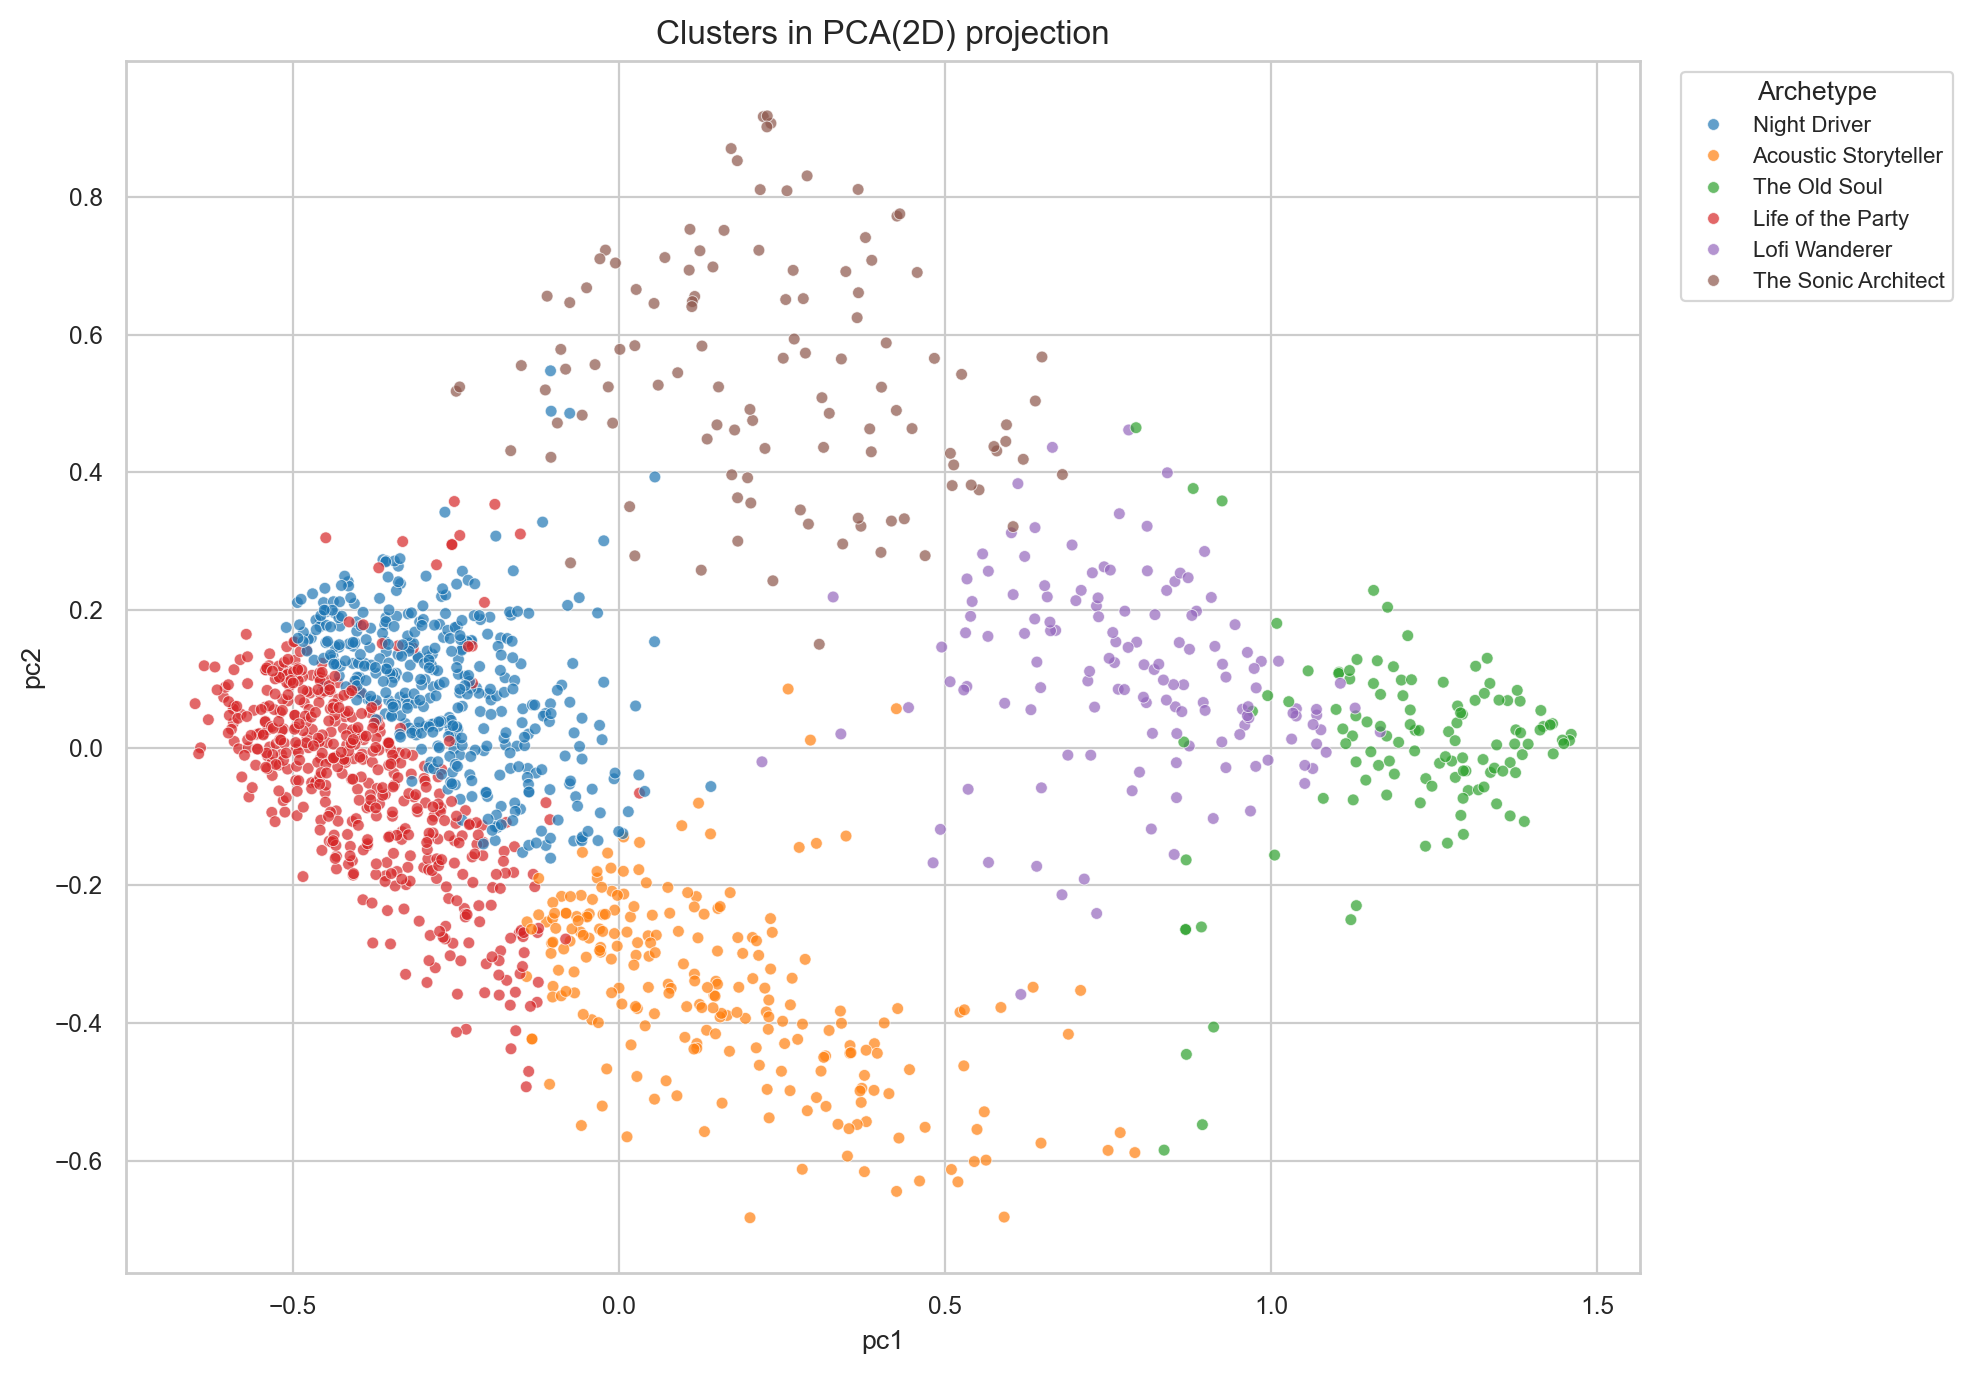
\includegraphics[width=0.48\textwidth]{figures/cluster_pca.png}
\caption{Clusters projected into PCA(2D). Acoustic/instrumental archetypes (Old Soul, Lofi Wanderer) separate cleanly from upbeat mainstream (Life of the Party, Night Driver).}
\label{fig:cluster_pca}
\end{figure}

\begin{figure}[h]
\centering
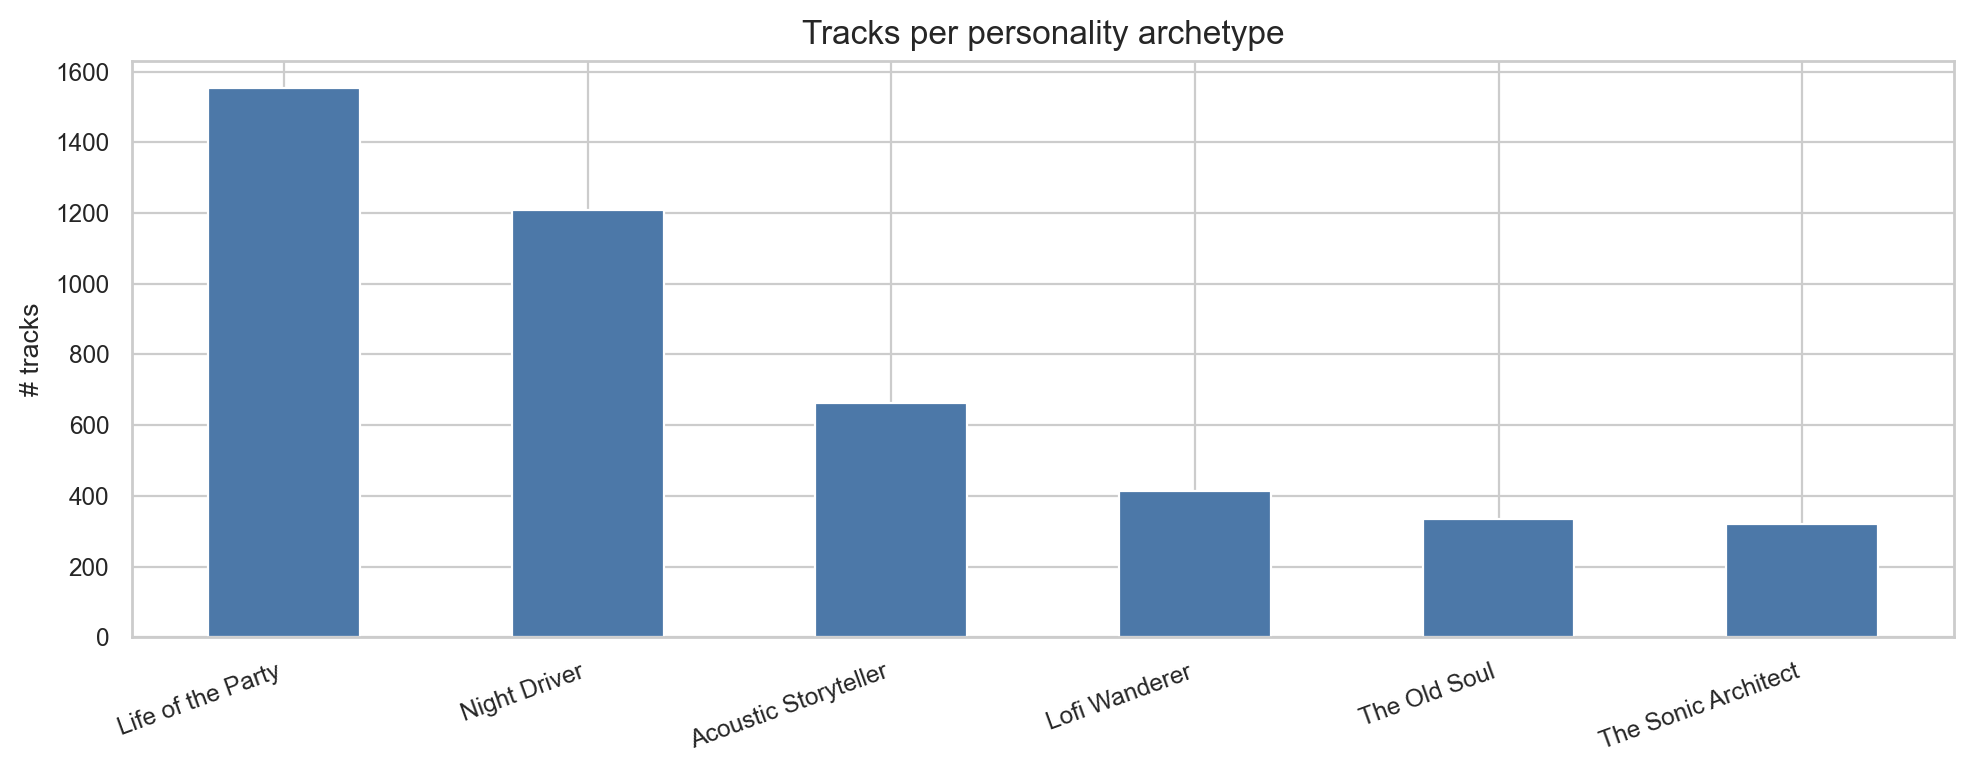
\includegraphics[width=0.48\textwidth]{figures/cluster_sizes.png}
\caption{Tracks per archetype. ``Life of the Party'' is the largest cluster (35\% of catalog) reflecting the dataset's mainstream-pop skew; the smallest is ``The Sonic Architect'' at 7\%.}
\label{fig:cluster_sizes}
\end{figure}

Centroid analysis (Fig.~\ref{fig:cluster_profile}, supported by per-cluster top-genre composition) yielded six interpretable archetypes:
\begin{itemize}
\item \textbf{Lofi Wanderer} --- high acousticness + instrumentalness, low energy. Lofi/jazz/world.
\item \textbf{Night Driver} --- low-acoustic, high-energy, low-valence. Moody mainstream.
\item \textbf{Life of the Party} --- highest danceability/valence/energy. Latin/pop/hip-hop. (1{,}553 tracks; 35\% of catalog.)
\item \textbf{The Old Soul} --- very low energy, very high acoustic+instrumental. Wellness/classical/ambient.
\item \textbf{The Sonic Architect} --- electronic instrumentals, deep house.
\item \textbf{Acoustic Storyteller} --- vocal acoustic mid-tempo. Latin/ambient/pop classics.
\end{itemize}

\subsection{Recommendation Engine}

The recommendation engine computes the user profile $\bar{x}$ and ranks all candidate tracks by the blended score
\begin{equation}
\text{final}(t) = \alpha \cdot \cos(t, \bar{x}) + (1-\alpha)\cdot \frac{\text{popularity}(t)}{100}
\end{equation}
returning the top-10. Cosine similarity is preferred over Euclidean for two reasons (validated in Section~\ref{sec:metric_compare}): it captures \emph{directional} alignment of taste profiles regardless of magnitude, and it admits the simple ``recommended because it has similar energy, valence, and danceability'' explanation.

\subsection{Hidden Gems}

Hidden gems use a strict similarity filter ($\alpha{=}1.0$) and an adaptive popularity ceiling. A track $t$ qualifies if its similarity is in the top decile and its popularity is below $\min(\text{median}(\mathcal{C}), \overline{\text{popularity}}(S))$. The adaptive ceiling handles two user types: mainstream listeners get tracks below the global median; niche listeners (whose own seed popularity is already low) get tracks below their own average. The Streamlit app additionally excludes any track already in the main rec list to keep the two surfaces disjoint.

\subsection{Streamlit Demo}

The demo is a single Streamlit page (\texttt{app/streamlit\_app.py}) with a sticky picker at top and six sequential slides below: (1) Music in Numbers (counts, top genres/artists), (2) Mood (label + valence/energy scatter against catalog backdrop), (3) Music Personality (archetype + cluster centroid radar), (4) Audio DNA (user vs.\ catalog mean radar), (5) Top Recommendations (ranked table), (6) Hidden Gems (lower-popularity matches). The catalog and the joblib personality artifact are loaded once via \texttt{@st.cache\_resource}; per-track genre labels are intentionally hidden from the rec/gems tables because the dataset's \texttt{playlist\_genre} is the genre of the source playlist, not the song's own genre, which produces visibly wrong per-track labels (e.g., a Lil Baby track appearing as ``arabic'' because it was scraped from a playlist named ``Arab X'').

\section{Experiments and Results}

\subsection{Setup}

All offline metrics were computed on 200 simulated users $\times$ 5 seed songs each (1{,}000 leave-one-out trials), under two seed-construction strategies: \emph{random} (5 uniformly-sampled tracks --- an eclectic listener) and \emph{genre-coherent} (5 tracks from a single playlist genre with $\geq 5$ tracks --- a focused listener). Both populations use the same 4{,}494-track catalog after Min--Max scaling.

\subsection{Leave-One-Out Seed Recovery}

For each seed, one song is held out, the user profile is rebuilt from the rest, and the held-out song's rank in the cosine-sorted catalog is recorded. Table~\ref{tab:loo} summarizes Hit@K, mean reciprocal rank (MRR), and rank statistics. Genre-coherent seeds achieve median rank 950 of 4{,}494 (2.4$\times$ better than the random baseline of 2{,}247), Hit@10 of 1.6\% (8$\times$ random), and MRR 0.0104. Random seeds score near the baseline because their average profile across five unrelated tracks is a meaningless midpoint.

\begin{table}[h]
\centering
\caption{Leave-one-out seed recovery (1{,}000 held-out trials per strategy).}
\label{tab:loo}
\begin{tabular}{lrrr}
\toprule
Metric & Random & Genre-coherent & Random baseline \\
\midrule
Hit@5 & 0.001 & 0.012 & 0.001 \\
Hit@10 & 0.001 & \textbf{0.016} & 0.002 \\
Hit@50 & 0.006 & 0.066 & 0.011 \\
MRR & 0.0015 & 0.0104 & --- \\
Median rank & 2{,}234 & \textbf{950} & 2{,}247 \\
Mean rank & 2{,}278 & 1{,}281 & 2{,}247 \\
Avg.\ recovered sim. & --- & 0.936 & --- \\
\bottomrule
\end{tabular}
\end{table}

\begin{figure}[h]
\centering
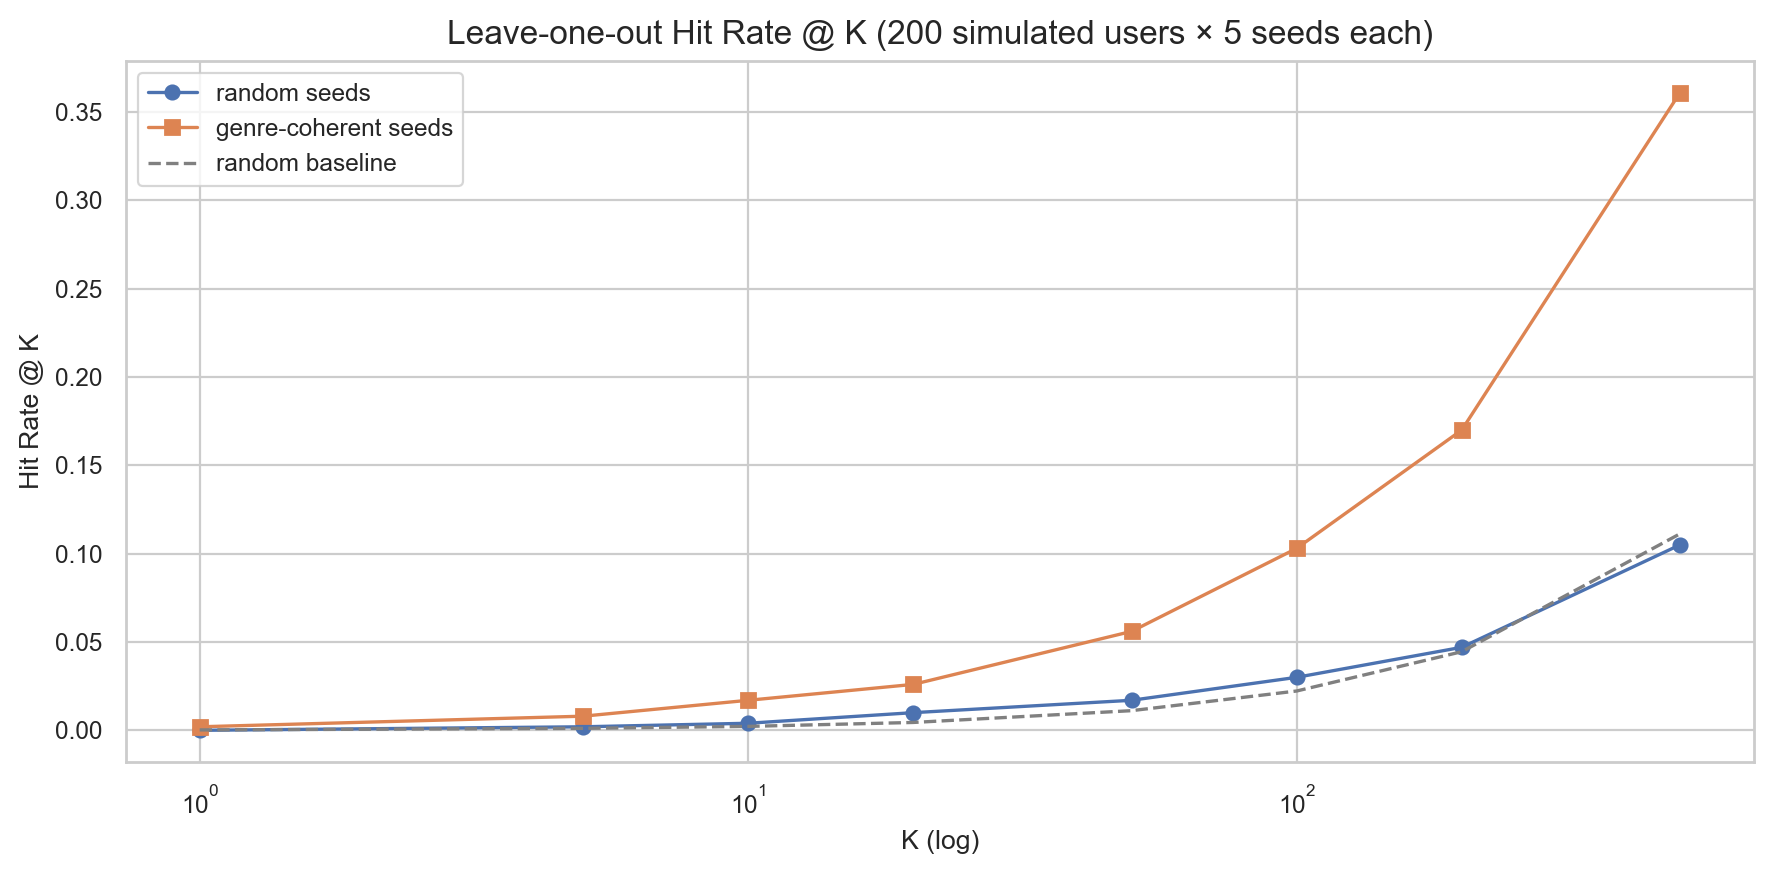
\includegraphics[width=0.48\textwidth]{figures/loo_hitrate.png}
\caption{Hit Rate @ K from leave-one-out, log K-axis. Genre-coherent seeds dominate the random baseline at every K; random-seed performance hugs the baseline because the average profile of unrelated tracks is meaningless.}
\label{fig:loo}
\end{figure}

The \texttt{avg\_recovered\_similarity} statistic --- 0.936 cosine similarity between the held-out track and the rebuilt 4-song profile --- is the §7.3 sanity check from the implementation plan: when a held-out song is at rank $\sim 950$, it is still 94\% similar to the profile. Rank inflation is dataset density (hundreds of near-identical tracks crowd the top), not recommender failure.

\subsection{Popularity-Blend Trade-off}
\label{sec:alpha}

We swept $\alpha \in \{1.0, 0.95, 0.85, 0.7, 0.5\}$ and measured genre consistency for both seed strategies (Fig.~\ref{fig:alpha}). For genre-coherent (focused) users, the textbook $\alpha{=}0.85$ default cuts genre consistency from 0.16 (pure cosine) to 0.08 --- a 47\% loss --- because the popularity term pulls recommendations toward the catalog's largest genres regardless of the seed. Random-seed users barely move (0.36 $\to$ 0.39) because their seed already spans many genres. We chose $\alpha{=}0.95$: a small popularity nudge for cold-start without crushing genre relevance.

\begin{figure}[h]
\centering
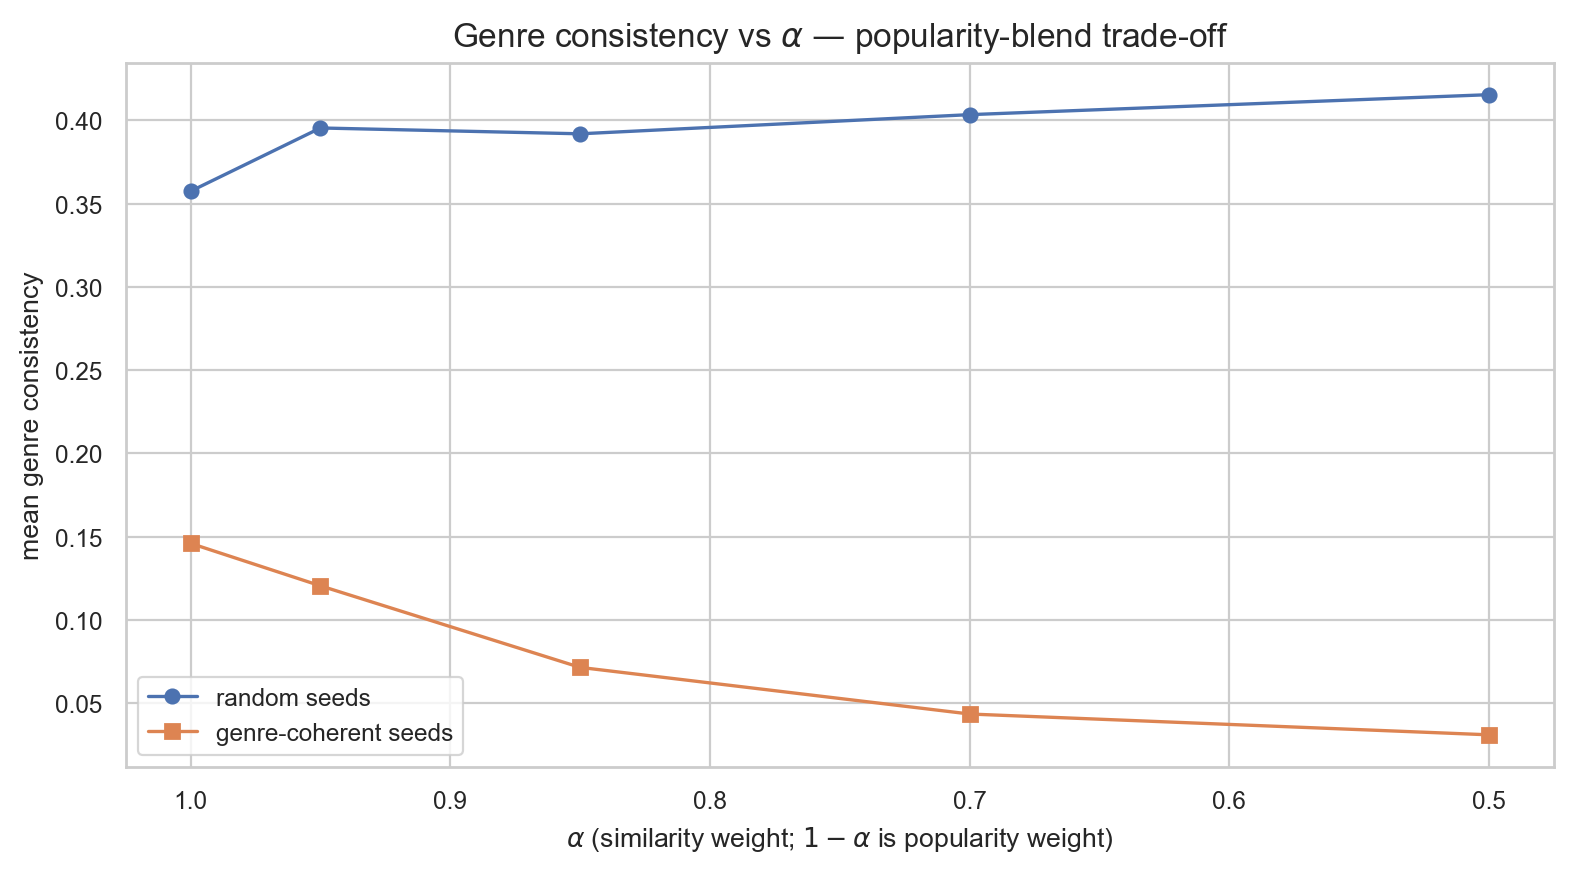
\includegraphics[width=0.46\textwidth]{figures/alpha_sweep.png}
\caption{Genre consistency vs.\ $\alpha$. Lower $\alpha$ (more popularity weight) hurts focused users more than eclectic ones. The chosen default is $\alpha{=}0.95$.}
\label{fig:alpha}
\end{figure}

\subsection{Cosine vs.\ Euclidean}
\label{sec:metric_compare}

The implementation plan §6 calls for a head-to-head comparison of the two distance metrics. We re-ran leave-one-out for genre-coherent seeds under both metrics (Table~\ref{tab:metric}, Fig.~\ref{fig:metric}). Cosine wins at the high-precision end (Hit@5 +20\%, Hit@10 +14\%, MRR +11\%) --- precisely where users actually look in a top-10 ranked list. Euclidean has a marginal edge in the tail (Hit@50, mean rank). The cosine win plus the directional-similarity explanation (``it points the same way in feature space'') justified retaining cosine.

\begin{table}[h]
\centering
\caption{Cosine vs.\ Euclidean on genre-coherent seeds (1{,}000 LOO trials).}
\label{tab:metric}
\begin{tabular}{lrrrr}
\toprule
Metric & Hit@5 & Hit@10 & MRR & Median rank \\
\midrule
\textbf{Cosine} & \textbf{0.012} & \textbf{0.016} & \textbf{0.0104} & \textbf{951} \\
Euclidean & 0.010 & 0.014 & 0.0094 & 989 \\
\bottomrule
\end{tabular}
\end{table}

\begin{figure}[h]
\centering
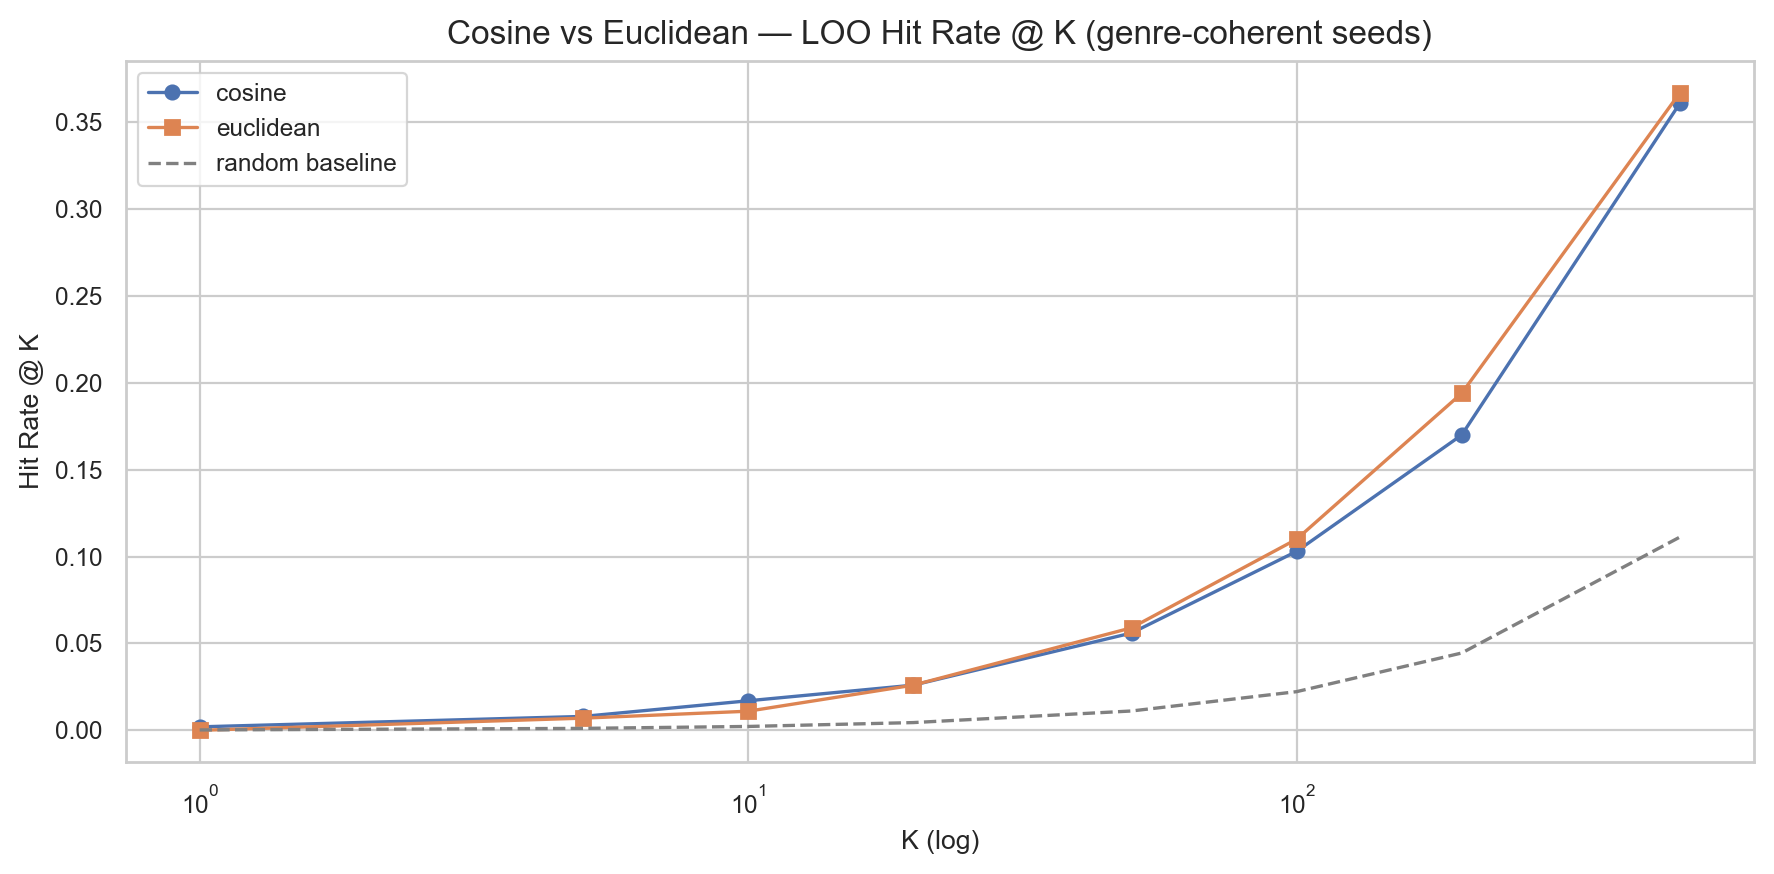
\includegraphics[width=0.48\textwidth]{figures/metric_comparison.png}
\caption{Cosine vs.\ Euclidean Hit Rate @ K (log K-axis). The two curves track closely; cosine's edge is concentrated in the small-K regime that drives a top-10 demo.}
\label{fig:metric}
\end{figure}

\subsection{Other Quality Metrics}

\emph{Intra-list diversity.} Mean pairwise cosine distance among the 10 recommended tracks is 0.03 (i.e., recommendations are 97\% mutually similar). This is expected for cosine on a dense feature space and is not necessarily a problem for music discovery, where similarity \emph{within} a profile is the desired behavior. A future maximal-marginal-relevance (MMR) re-ranking step could add diversity if needed.

\emph{Hidden-gem disjointness.} With the explicit \texttt{exclude} filter, gems and main recommendations have $\sim$0.0\% overlap by construction; without it, overlap was 50\%+ at $\alpha{=}0.95$ because the two surfaces were both similarity-driven.

\emph{Cluster stability.} Across five different K-means random seeds at $K{=}6$, silhouette score had standard deviation $9 \times 10^{-5}$ --- the clustering is initialization-stable.

\subsection{Limitations}

\textit{No user behavior data.} The catalog has no ratings or listening histories, so no collaborative filtering. Cold-start is handled by requiring seed selection.

\textit{Dataset density.} 4{,}494 tracks crammed into $[0,1]^8$ make absolute Hit@10 numbers small (1.6\% even for focused users) because hundreds of tracks have near-identical similarity to any profile. The recommender is correct directionally but not precise in absolute rank.

\textit{Noisy genre labels.} \texttt{playlist\_genre} tags each track with the genre of the playlist it was scraped from, not the song's own genre. We explored four corrections (album-majority, artist-majority, hybrid, agreement-only); each had distinct failure modes (album-majority misses single-track albums, artist-majority overrides correctly-labeled tracks). The pragmatic decision was to hide per-track genre from the demo's recommendation/gems tables; aggregate genre summaries (slide 1) are kept because noise averages out across the user's selection.

\textit{Equal feature weighting.} K-means and cosine treat all eight features equally. Weighted cosine (variance-inverse over the seed) is documented as a stretch goal.

\subsection{Future Work}

\begin{itemize}
\item \textbf{Weighted cosine similarity:} weight features by inverse variance over the seed, so a user picking 5 high-energy songs has energy weighted more heavily.
\item \textbf{GMM personality:} replace hard K-means assignment with Gaussian Mixture Model soft labels (e.g., ``60\% Night Driver, 30\% Lofi Wanderer'').
\item \textbf{Mood trajectory playlists:} sequence songs along a calm-to-upbeat curve.
\item \textbf{Popularity prediction residuals:} regress popularity on audio features, use residuals to identify systematically under-popular tracks as hidden gems.
\item \textbf{Live Spotify API integration:} replace the static CSV with a real-time catalog and add 30-second audio previews to the demo.
\end{itemize}

\section{Conclusion}

A Wrapped-style framing turns a baseline content-based recommender into a complete data-mining demo. K-means at $K{=}6$ produced six interpretable music-personality archetypes; cosine-similarity ranking with a small ($\alpha{=}0.95$) popularity nudge beat Euclidean distance in top-K precision; hidden gems work as designed thanks to the adaptive popularity ceiling. The system is honest about its limitations: cosine on eight audio features is a weak ranker in absolute terms, but the per-archetype radar charts, the mood quadrant scatter, and the live song-pick interface make the result legible and engaging --- which is the actual point.

\bibliographystyle{IEEEtran}
\bibliography{IEEEabrv, references}

\end{document}
